\documentclass[cs4size,a4paper,nofonts]{ctexart}
\usepackage[utf8]{inputenc}
\def\tjf{{\tt{田劲锋}}}
\def\titlec{Linux常用工具的使用(2):文本编辑器的使用}
\usepackage[a4paper,margin=2.2cm]{geometry} % 页面设置
\usepackage[unicode,breaklinks=true,
colorlinks=true,linkcolor=black,anchorcolor=black,citecolor=black,urlcolor=black,
pdftitle={\titlec},pdfauthor={\tjf}]{hyperref}
%\CTEXsetup[number=\chinese{section}, format={\large\sf\bfseries}]{section}
\usepackage{latexsym,amsmath,amssymb,bm}
\usepackage{graphicx}
\usepackage{subfigure}
\usepackage{wrapfig}
\usepackage{fancyvrb}
\DefineShortVerb{\|}
\fvset{frame=single}

\setmainfont{Times New Roman}
\setCJKmainfont[BoldFont={SimHei}]{SimSun}  % 主要字体:宋体、黑体
\setCJKsansfont[BoldFont={STZhongsong}]{STFangsong} % 次要字体:仿宋、中宋
\setCJKmonofont{KFKai} % 等宽字体:楷体

\CJKsetecglue{\hspace{0.1em}}
\renewcommand\CJKglue{\hskip -0.3pt plus 0.08\baselineskip}
\frenchspacing
\widowpenalty=10000
\linespread{1.2} % 行距

\usepackage[inline]{enumitem} % 调整列表样式
\setlist{noitemsep,align=left}
%\setlist[itemize]{topsep=0pt,partopsep=0pt,itemsep=0pt,parsep=0pt}
\setlist[enumerate]{topsep=0pt,partopsep=0pt,itemsep=0pt,parsep=0pt}
\setlist[enumerate,1]{label={(\arabic*)}}
\setlist[enumerate,2]{label={\arabic*)}}

\CTEXsetup[beforeskip={0pt},afterskip={0pt}]{paragraph}

%\makeindex
\pagestyle{plain}

\begin{document}

%%%% 开始 %%%%

\begin{titlepage}

\begin{center}


\includegraphics[height=1cm]{image/haut.png}

\vspace*{1cm}
{\liti\fontsize{48pt}{50pt}{课\quad 程\quad 设\quad 计}}

\vspace*{4cm}
{\fontsize{36}{80}\sf\bfseries \titlec}

\vspace*{1cm}
{\fontsize{30}{70}\sf\bfseries \titlee}

\vfill
{\large
\newcommand{\ctline}[2]{\makebox[6em][s]{\bf #1}:\underline{\makebox[14em][c]{\qquad #2\qquad}}\\}
\ctline{课程设计名称}{数据结构课程设计}
\ctline{专业班级}{计算机 1303 班}
\ctline{学生姓名}{\tjf}
\ctline{学号}{201316920311}
\ctline{指导教师}{白\quad 浩}
\ctline{课程设计时间}{\today}
}

\end{center}

\end{titlepage}


% \CTEXnoindent

\paragraph{实验题目:}\titlec

\paragraph{实验目的:}
(1)理解文本编辑器vi的工作模式;(2)掌握文本编辑器的使用方法

\paragraph{实验内容:}
\begin{enumerate}
\item 阐述vi编辑器的3种工作模式,以及如何实现工作模式的互相转换?
\item 在文本编辑器vi中,实现下列功能,列举出一个例子即可:
\begin{enumerate}
\item 添加单个字符、多个字符
\item 删除单个字符、删除整行文本
\item 文本的替换
\item 文本的复制和粘贴
\item 文本的剪切和粘贴
\item 全文关键字查找
\item 全文字符串替换
\item 保存、另存为、退出
\item 同时打开两个文件,实现两个窗口的切换
\item 区域复制
\item 与shell交互
\end{enumerate}
\end{enumerate}

\paragraph{实验步骤:}\quad

\newcommand{\image}[3][width=\textwidth]{
  \begin{minipage}[t]{0.5\textwidth}
    \centering
        \includegraphics[#1]{images/exp5/#2.png}
    \caption{#3}
    \label{fig:#3}
  \end{minipage}
}

这里我使用运行在 Mac OS X 上终端下的 Vim。

\begin{enumerate}

\item Vim常用三个模式:命令模式、插入模式、可视模式。

在命令模式下,用|h j k l|左下上右移动光标,|w e b|移动到单词首尾,\verb+0 ^ $+移动到行首尾,|gg G|移动到文档首尾。

|yy|复制行,|yw|复制单词,|p P|粘贴,|dd dw D x|剪切。命令前加数字可以重复。

进入插入模式用|i|,或者|a|从光标后插入,|o O|另起新行,|I A|插入到行首尾。

用|Esc|退出插入模式。

可视模式不常用,按|v|进入,可以选择文本。

冒号指令|:w|保存,|:e|编辑,|:q|退出,|:x|保存并退出。

|/pattern|查找,\verb+:%s/find/replace/g+替换。

\item 这里我以编辑本次实验报告为示例,来完成本次实验。

\end{enumerate}

\begin{figure}[htp]
\centering
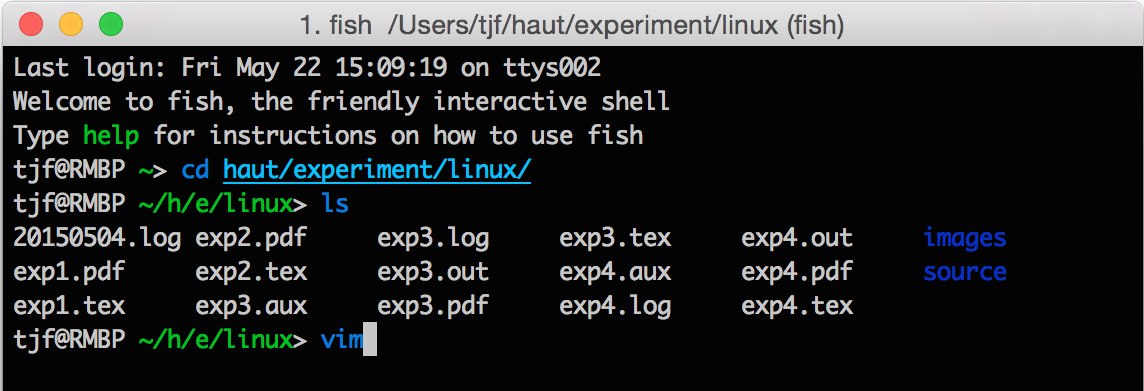
\includegraphics[width=10cm]{images/exp5/1.start.png}
\caption{启动Vim}
\label{fig:启动Vim}
\end{figure}

如图\ref{fig:启动Vim},首先在终端中键入|vim|以启动Vim。

\begin{figure}[htp]
\image{2.read}{读入实验四}
\image{3.saveas}{保存为实验五}
\end{figure}

我要编写的是实验五的实验报告,这里直接读入实验四的内容进行修改。如图\ref{fig:读入实验四},将实验四的\LaTeX 源文件读入进来。如图\ref{fig:保存为实验五},键入|:w exp5.tex|,将当前编辑的文稿另存为实验五。

\begin{figure}[htp]
\image{4.paste}{从外部粘贴}
\image{5.indent}{自动缩进}
\end{figure}

接着将光标移动到待修改的地方,这里是实验目的和实验内容,用|dd|删除这里原有的内容后,按|i|进入插入模式,从老师给出的Word文档中复制这段文字,粘贴进来。如图\ref{fig:从外部粘贴},Vim将直接粘贴进来的文本做了不好的缩进。在命令模式下将光标移动到段首,输入|13==|将55--67行的文本自动缩进,如图\ref{fig:自动缩进}。

\begin{figure}[htp]
\image{6.select}{选择文本块}
\image{7.insert}{批量插入}
\end{figure}

光标定位到58行,按下|CTRL-v|进入可视块模式,如图\ref{fig:选择文本块},按|11j|向下选择11行,按|3l|向右选择3列。这里我要将这些文本编号改写成\LaTeX 的格式,键入|I|进入插入模式,输入|\item |之后,连续按两下|Esc|键,Vim将自动填充到选择的文本块中,如图\ref{fig:批量插入},实现了批量插入的功能。

\begin{figure}[htp]
\image{8.delete}{删除到指定行}
\image{9.vsplit}{分割窗口}
\end{figure}

\begin{figure}[htp]
\image{10.copy}{复制文本}
\image{11.cc}{调用Shell}
\end{figure}

接下来将实验四的实验内容全部删除,按|G|跳转到文件尾,查看到实验内容最后一行的行号为215,然后跳转到实验内容第一行(这里是第84行),键入|d:216|从当前光标处删除到第216行,如图\ref{fig:删除到指定行},中间的内容全部被删除。

使用分割窗口的功能,键入|:vsplit ../os/exp1.tex|打开操作系统实验一的源文件,如图\ref{fig:分割窗口}。打开后如图\ref{fig:复制文本}是竖屏分割的,光标移动到相应位置,按|15yy|将操作系统实验中关于Vim描述的15行文字复制下来,按两下|CTRL-w|切换窗格,光标跳转到Linux实验中相应位置,按|p|粘贴。

使用|:tabnew|可以打开一个新的标签页,这里我打开了操作系统实验一的一个C程序源文件。如图\ref{fig:调用Shell},键入
\begin{Verbatim}
!cc ../os/exp2/parent_child.c
\end{Verbatim}
来调用Shell解释程序,执行clang编译器,将该源文件编译成可执行文件|a.out|,Vim会跳转回终端显示相应信息。键入
\begin{Verbatim}
!./a.out
\end{Verbatim}
调用Shell来执行这个编译后的程序。

\begin{figure}[htp]
\image{12.find}{查找文本}
\image{13.replace}{替换文本}
\end{figure}

如图\ref{fig:查找文本},键入
\begin{Verbatim}
/main
\end{Verbatim}
来查找“main”出现的位置。

如图\ref{fig:替换文本},键入
\begin{Verbatim}
:%s/process/进程/g
\end{Verbatim}
将文件中所有“process”替换成“进程”。

\vspace*{1em}

\paragraph{实验体会:}\quad

这次实验是关于|vi|的使用,实际上|vi|有一些微妙的地方并不是很好用,所以一般都会使用增强版的Vim来代替|vi|。我这里的Vim是经过配置,有代码高亮和行号显示的。Vim的学习曲线是比较长的,虽然我用Vim也有很多年了,但也并不完全熟悉其强大功能。当然,有什么不会的看看帮助文档和用户手册,问题也就好解决了。

\end{document}
